\section{Event: addEventListener, Objek Event, dan Propagation}

\code{addEventListener(type, handler)} mendaftarkan fungsi yang dipanggil saat event tertentu terjadi pada elemen. Berbeda dari atribut HTML (\code{onclick="..."}), \code{addEventListener} memungkinkan \textbf{multiple handlers} pada satu elemen dan mendukung phase capturing. Parameter ketiga opsional: \code{true} untuk capturing phase, atau objek opsi \code{\{capture, once, passive\}} \cite{jsInfo}.

\begin{figure}[htbp]
\centering
\resizebox{0.7\textwidth}{!}{%
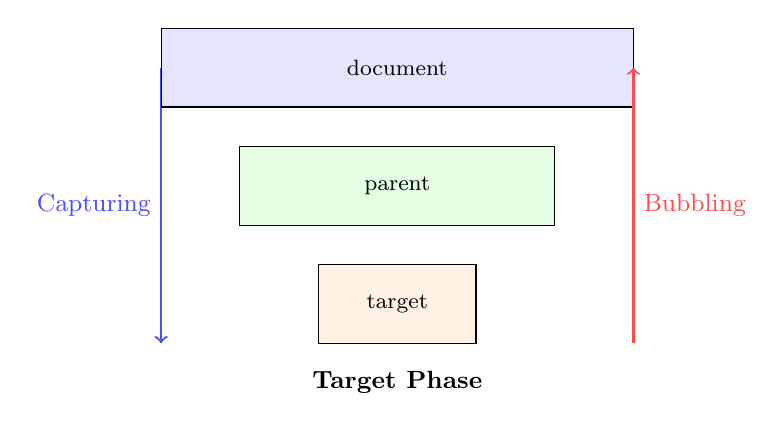
\begin{tikzpicture}[every node/.style={font=\footnotesize}]
  % Phases
  \draw[thick, blue!70, ->] (0,4) -- (0,0.5) node[midway, left, font=\small] {Capturing};
  \node[draw, fill=blue!10, minimum width=6cm, minimum height=1cm] at (3,4) {document};
  \node[draw, fill=green!10, minimum width=4cm, minimum height=1cm] at (3,2.5) {parent};
  \node[draw, fill=orange!10, minimum width=2cm, minimum height=1cm] at (3,1) {target};
  \draw[thick, red!70, ->] (6,0.5) -- (6,4) node[midway, right, font=\small] {Bubbling};
  \node[font=\small\bfseries] at (3,0) {Target Phase};
\end{tikzpicture}%
}
\caption{Event propagation: capturing (turun) $\rightarrow$ target $\rightarrow$ bubbling (naik)}
\end{figure}

\begin{table}[htbp]
\centering
\scriptsize
\begin{tabular}{|P{3.5cm}|P{2.4cm}|P{2.6cm}|}
\hline
\textbf{Properti Event} & \textbf{Tipe} & \textbf{Kegunaan} \\
\hline
\code{event.target} & Elemen asal & Elemen yang diklik \\
\hline
\code{event.current\-Target} & Elemen listener & Elemen yang punya handler \\
\hline
\code{event.type} & String & Jenis event (\code{"click"}) \\
\hline
\code{event.}\linebreak[0]\code{preventDefault()} & Method & Batalkan aksi default \\
\hline
\code{event.stop}\linebreak[0]\code{Propagation()} & Method & Hentikan bubbling \\
\hline
\end{tabular}
\caption{Properti objek Event yang sering digunakan}
\end{table}

\begin{konsep}
\textbf{Event Delegation.} Alih-alih memasang listener di setiap item, pasang satu listener di parent dan periksa \code{event.target}: \code{list.addEventListener("click", e => \{ if (e.target.matches("li")) handleClick(e.target); \})}. Ini efisien untuk daftar dinamis (item yang ditambah/hapus) dan mengurangi jumlah listener \cite{mdnJsGuide}.
\end{konsep}

